% NOTE:
% latexmk -shell-escape -pvc slides.tex # Watches and compiles on each change.
% latexmk -c slides.tex   # Clean the temporal files.

\documentclass[20pt]{beamer}

% Adapted from;
% How to Design a Scientific Poster using Beamer -1 (Latex Basic Tutorial-30)
% https://youtu.be/2ZWnFFhVkdE?si=N3e1Ob8YWyTwW19e

\usepackage[size=custom, width=90, height=120, orientation=portrait, scale=1.4]{beamerposter}
\usetheme{Madrid}
\usepackage{changepage}
\usepackage[numbers]{natbib}
\usepackage{listings}
\usepackage{siunitx}
\usepackage{hyperref}
\usepackage[linesnumbered,algoruled,longend]{algorithm2e}
\usepackage{graphicx}
\usepackage{subcaption}

\beamertemplatenavigationsymbolsempty

\renewcommand{\raggedright}{\leftskip=0pt \rightskip=0pt}
\let\olditemize\itemize
\renewcommand{\itemize}{\olditemize\addtolength{\itemsep}{0.4\baselineskip}}

\addtobeamertemplate{block begin}{}{\vspace{5mm}\begin{adjustwidth}{5mm}{5mm}}
\addtobeamertemplate{block end}{\end{adjustwidth}\vspace{10mm}}{\vspace{5mm}}

\setbeamertemplate{caption}[numbered]

\setbeamerfont{block title}{size={\centering\bfseries\fontsize{48}{60}}}
\setbeamercolor{block body}{bg=white}
\setbeamercolor{background canvas}{bg=white}
%\definecolor{title-color}{RGB}{127, 96, 0}
\setbeamercolor{fbcolor}{fg=white, bg=cyan}
\setbeamertemplate{headline}{
    \begin{beamercolorbox}[wd=\paperwidth]{fbcolor}\vskip5mm
        \begin{columns}
            \begin{column}{0.20\linewidth}
            \centering
            
\includegraphics[width=0.65\linewidth]{logos/trees-color-h_2.png}
            \end{column}
            \begin{column}{0.60\linewidth}
            \centering\bfseries
\fontsize{80pt}{96}\selectfont A tool for prioritizing deforestation hotspots in the Brazilian Amazon \\ [6mm]
{\fontsize{48pt}{60}\selectfont 
\underline{Alber Sanchez}${}^1$, Guilherme Mataveli${}^1$, Gabriel de Oliveira${}^2$, \\
Michel E. D. Chaves${}^{1,5}$, Ricardo Dalagnol${}^3$, Fabien H. Wagner${}^3$, \\
Celso H. L. Silva Junior${}^4$, Luiz E. O. C. Aragao${}^1$ 
\\}
\vspace{10mm}
{\fontsize{38}{48}\selectfont ${}^1$National Institute for Space Research, Brazil; ${}^2$University of South Alabama, USA;${}^3$University of California, USA; ${}^4$State University of Maranhão; ${}^5$São Paulo State University in Tupã, Brazil.\\} 
%\vspace{1mm}
{\fontsize{44}{54}\selectfont alber.ipia@inpe.br}
            \end{column}
            \begin{column}{0.20\linewidth}
            \centering
            
\includegraphics[width=0.90\linewidth]{logos/geoinfo_2023.png}
            \end{column}
        \end{columns}\vskip5mm
    \end{beamercolorbox}
    %\color{blue}\rule{\paperwidth}{10pt}
}

\setbeamercolor{footcolor}{fg=white, bg=black}
\setbeamertemplate{footline}{
    \begin{beamercolorbox}[wd=\paperwidth, center, ht=1.5em]{footcolor}
        \small Any questions or suggestions? Write to alber.ipia@inpe.br
    \end{beamercolorbox}
}

\begin{document}\vspace*{-2cm}
\begin{frame}[fragile,t]
\begin{columns}[t]


%==== Column 1 ====
\begin{column}{0.33\linewidth}
\vspace{1cm}
    \begin{block}{Introduction\vphantom{g}}
    
Despite deforestation reduction promises by different governments, no administration has achieved zero illegal deforestation~\cite{dearealeaopereira2019}.
Deforestation policies and their enforcement are subject to government changes, challenging long-term environmental planning. 
As a result, deforestation in the Brazilian Amazon has had a positive trend since 2012 (See Figure~\ref{fig:deforestation_prodes}).

\vspace{1cm}
\begin{figure}[ht]
\centering
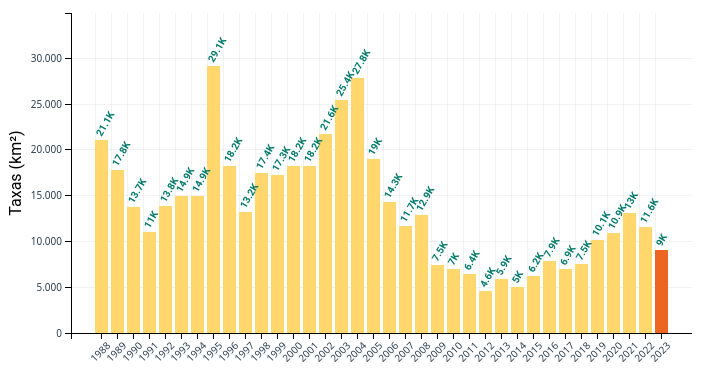
\includegraphics[width=0.9\textwidth]{fig_poster/taxa_desmatamento_2023.png}
\caption{Deforestation in the Brazilian Amazon (\unit{\km\squared}). Source \href{http://terrabrasilis.dpi.inpe.br}{INPE}.}
\label{fig:deforestation_prodes}
\end{figure}
\vspace{1cm}

We believe that policies regarding deforestation should be subject to public scrutiny and based on scientific principles. 
For this reason, we proposed an index for prioritizing areas in the Brazilian Amazon for law enforcement actions (check \emph{"Science‐based planning can support law enforcement actions to curb deforestation in the Brazilian Amazon"}~\cite{mataveli2022}).
Our index is on based variables aggregated into a regular grid of 25x25 km, 2019 to 2023 using the Random Forest algorithm~\cite{mataveli2023}.

To ensure the openness and transparency of our proposal, we prepared a data and software bundle using the \textit{R} language (hereby called package) that allows the public and other research teams to reproduce our methods and findings. This package is what we show here.

    \end{block}


\vspace{1cm}
    \begin{block}{Scientific reproducibility with \textsf{R}}

According to the Association for Computing Machinery (ACM) badging system, there are three types of reproducibility~\cite{acm2020}:
\begin{itemize}
\item Repeatability. Research teams can reliably repeat their computations. 
\item Reproducibility. Independent research teams can obtain the same results using the authors' software.
\item Replicability. Independent research teams obtain the same results using their own artifacts.
\end{itemize}

\textit{R} is a programing (scripting) language for statistical computing and graphics~\cite{rlanguage}.
\textit{R} is extensible through packages, which enable it  to load and run code, data, demos, examples, documentation, tests, and consistency checks~\cite{wickham2015}, making it well suited for distributing scientific results~\cite{pebesma2012}.

Since the inception of our index and paper, \textit{R} packages have allowed us to achieve both repeatability and reproducibility. 
The former was because the code and data required to run our experiment were packaged as a single unit, and the latter was because by making our package available online (see Links below), we allowed reproducibility. 
Because replicability depends on independent research groups, their own data, and their own software, it cannot be achieved.



    \end{block}
\end{column}



%==== Column 2 ====
\begin{column}{0.33\linewidth}
\vspace{1cm}
    \begin{block}{Results\vphantom{g}}
    \label{sec:results}
    
\begin{figure}[ht]
\centering
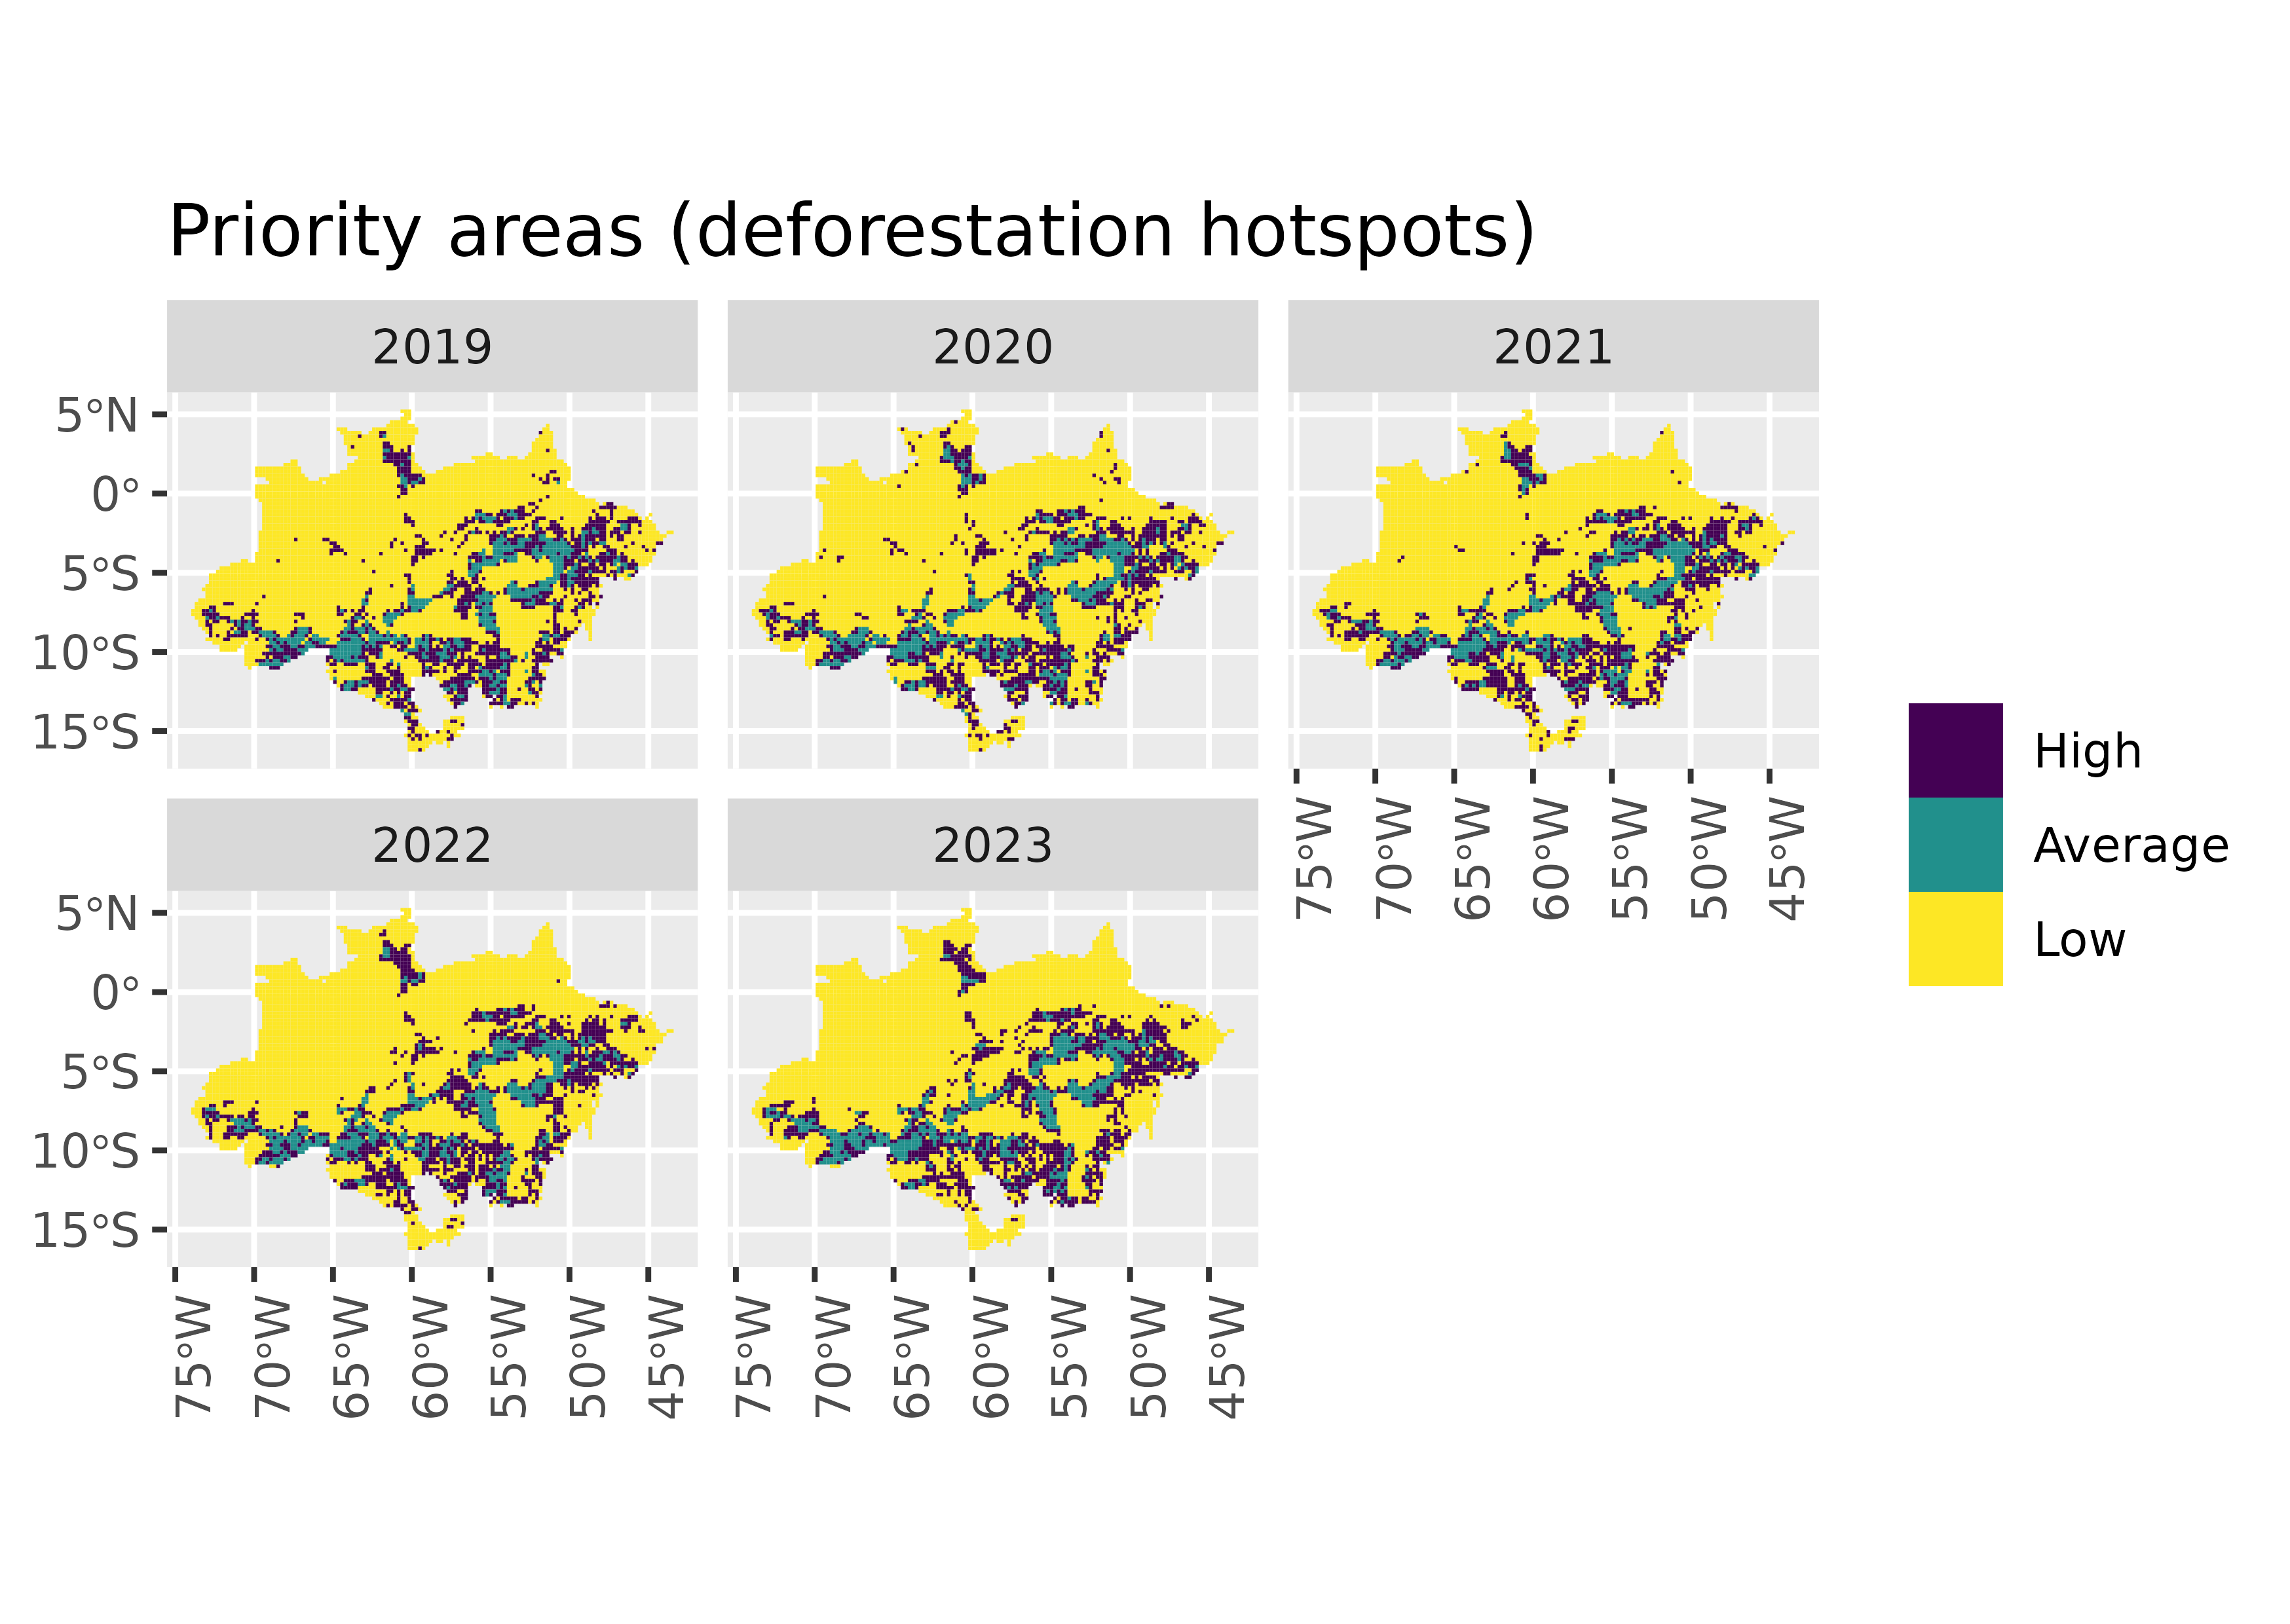
\includegraphics[width=0.9\textwidth,trim={0 1cm 0 2cm},clip] 
{figures/plot_results_precomputed.png}
\caption{Prioritization index as stored in our package.}
\label{fig:plot_results_precomputed}
\end{figure}

    \end{block}
    
\vspace{1cm}
    \begin{block}{Package description}
\label{sec:package}

Our package bundles both the code and the data required to prioritize deforestation areas for 2022 and 2023, allowing users to reproduce the results presented in our paper~\cite{mataveli2022} and its update~\cite{mataveli2023} (see Figure~\ref{fig:plot_results_precomputed}). 

Our package is available online (see Links below).

The code in this package fits the model presented in our paper (\textit{fit\_model()}) and estimates its accuracy (\textit{estimate\_accuracy()}), which is achieved by adjusting 100 models' data and then cross-validating them.
An additional function (\textit{results\_to\_shp()}) applies thresholds to the results to turn them into categories (e.g. low, average, and high) and exports them to a vector file compatible with GIS software.
These functions take only one parameter, the output directory (\textit{out\_dir}).

The results are the cross-validation models along with their metrics and error estimates, and 
the final model and its estimations. 
These results are stored in the R data format, CSV files, and GeoPackage files.

We ran our code using \textsf{R} 4.3.1 and GNU/Linux Ubuntu 20.04.6 (Kernel 5.15.90.1) LTS on top of Windows 10 Subsystem for Linux 1.2.5.0. 
We used 16 of the 32 available cores in an Intel Xeon E5-2640 v3 2.593~GHz processor with 32 GB of memory.
Given these software and hardware, \textit{fit\_model} took 13 minutes to run (user 9535.76, system 129.55, elapsed 752.90),  \textit{results\_to\_shp} took 14 hours (user 640670.17, system 10554.66, elapsed 50190.13), and \textit{results\_to\_shp} took a second (user 0.91,  system 0.02, elapsed 0.972).

Regarding data, our package includes 
a grid of 25~\unit{\km\squared} resolution, the pre-computed index (see Figure~\ref{fig:plot_results_precomputed}),
and the variables required by our model. 
This includes areas of deforestation, indigenous or protected lands; distances to waterways, highways, deforestation; and the number of fire spots (see Figure~\ref{fig:plot_fires}).

\vspace{1cm}
\begin{figure}[ht]
\centering
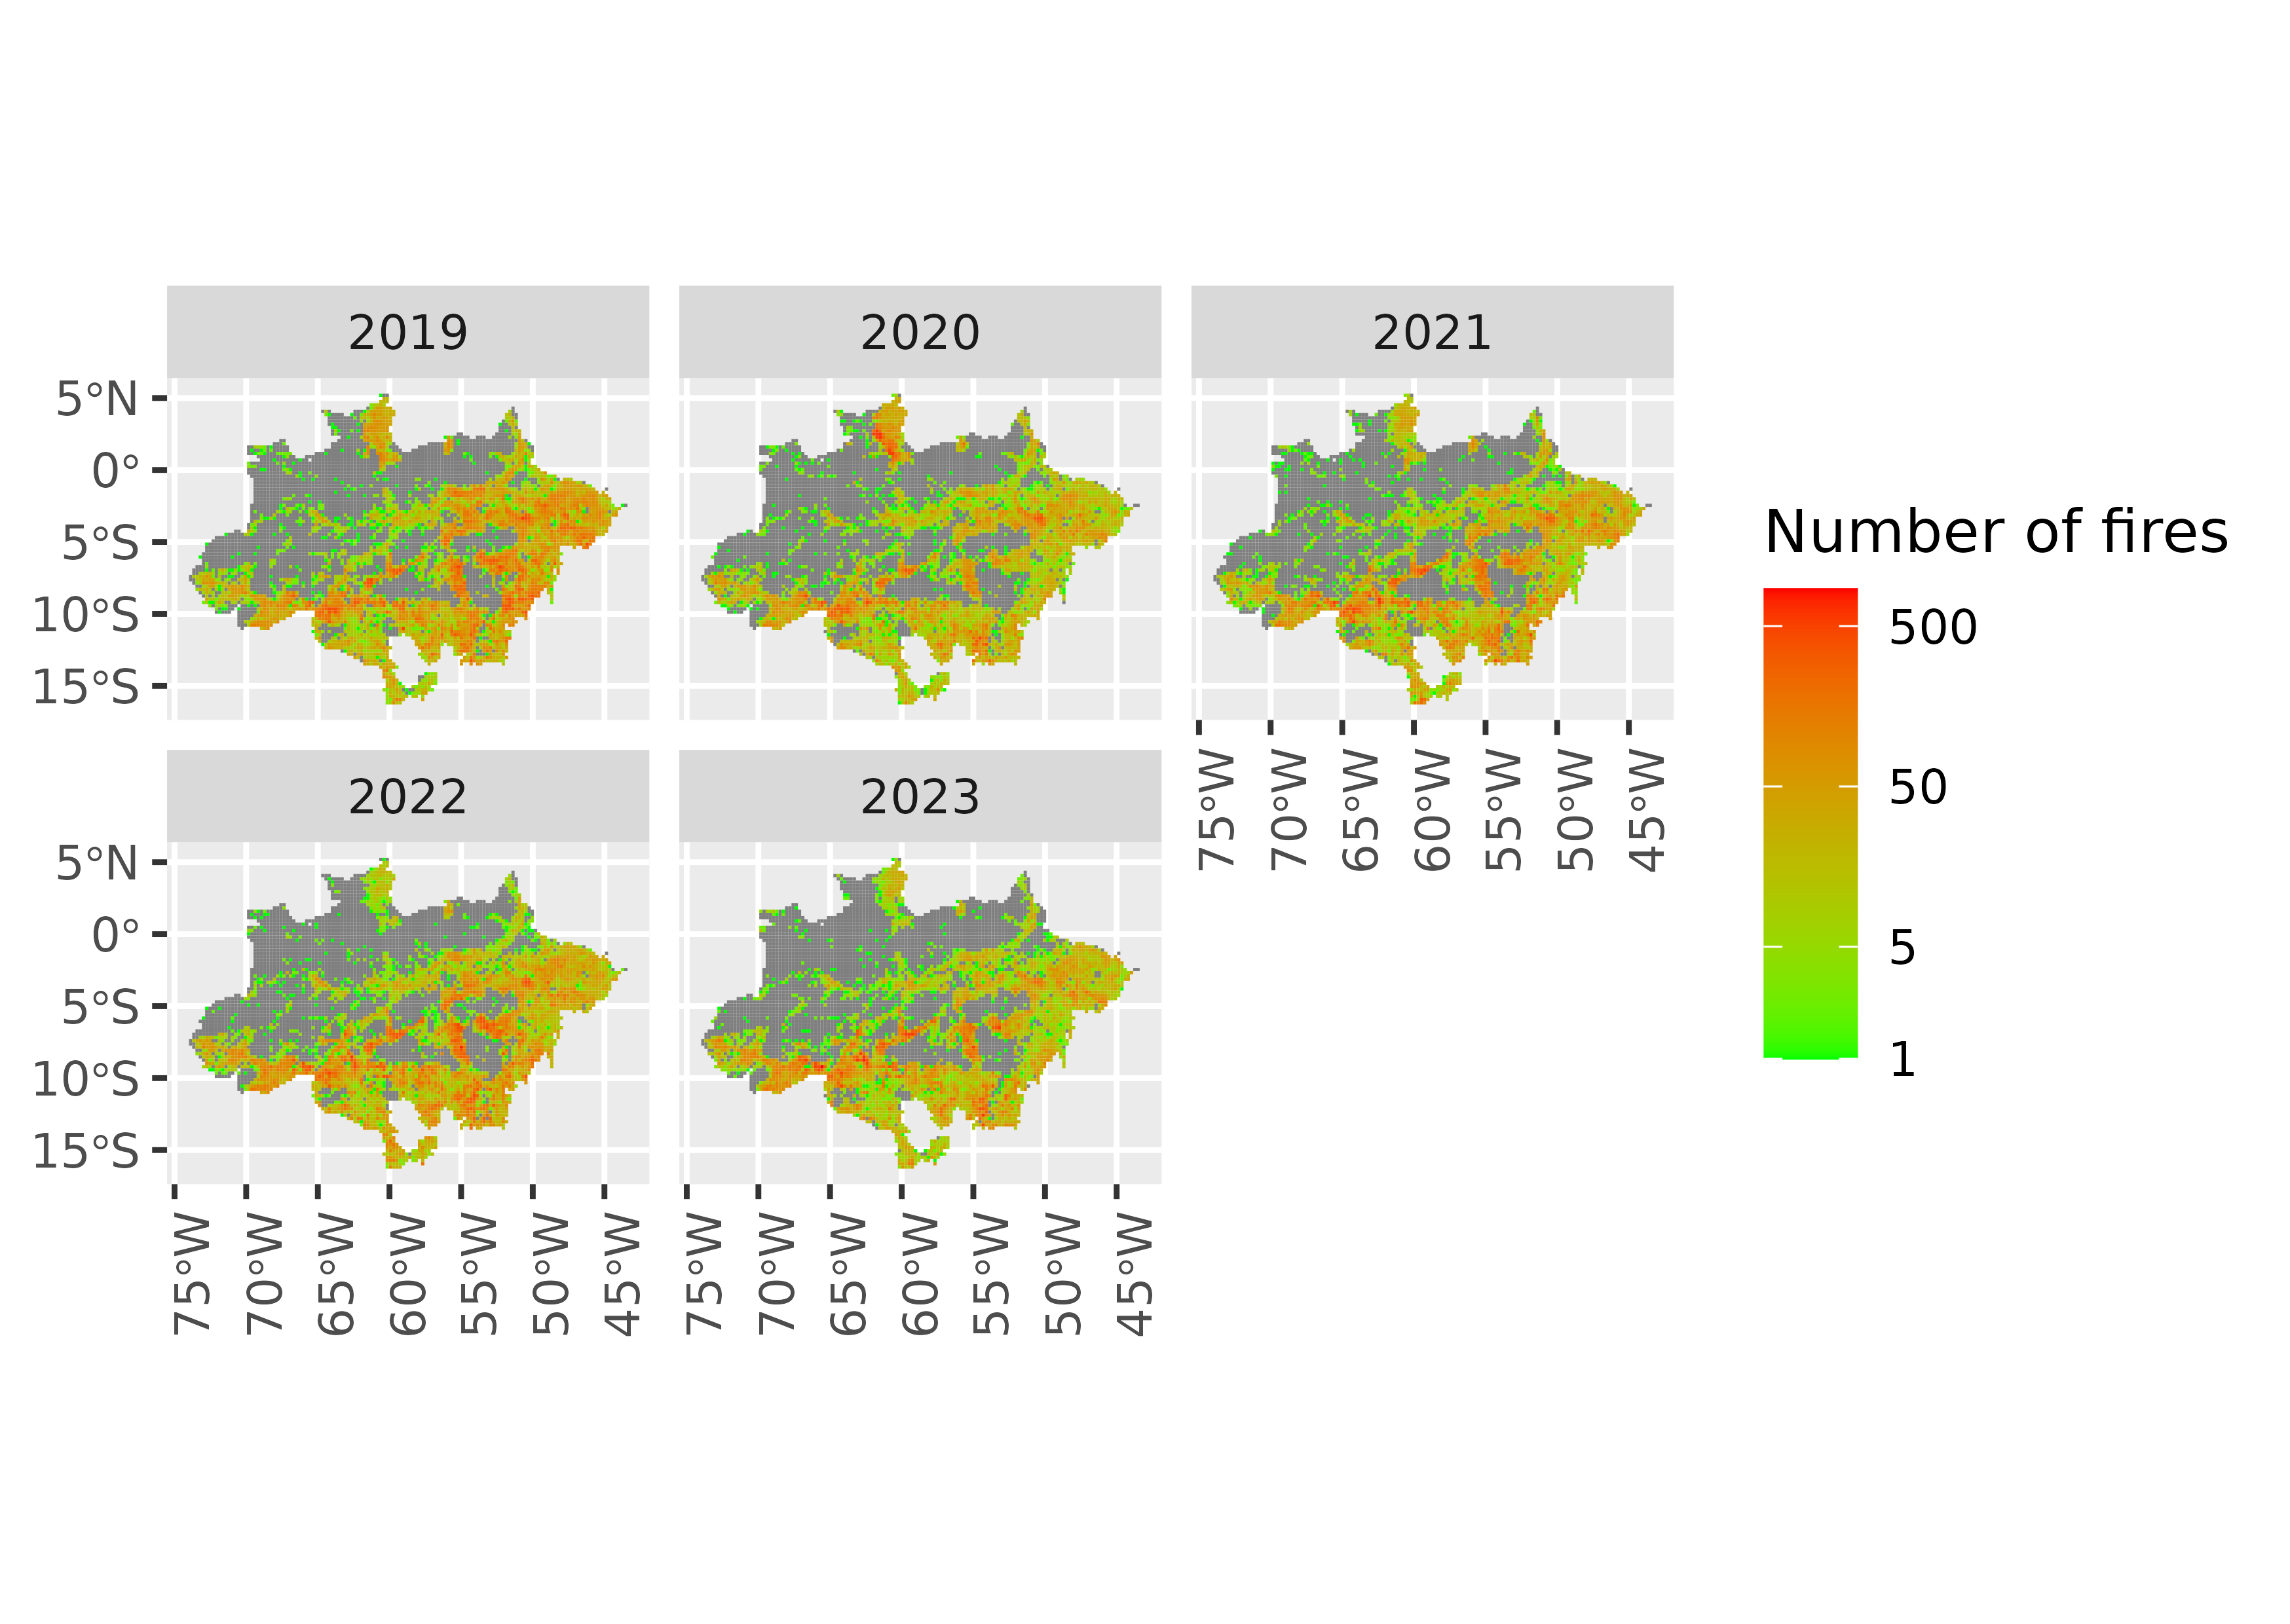
\includegraphics[width=0.9\textwidth,trim={0 1cm 0 2cm},clip] 
{fig_poster/plot_fires.png}
\caption{Number of fires. One of the variables for computing out prioritization index.}
\label{fig:plot_fires}
\end{figure}
\vspace{0.6cm}


   
    \end{block}
\end{column}






%==== Column 3 ====
\begin{column}{0.33\linewidth}
\vspace{1cm}
    \begin{block}{Final remarks\vphantom{g}}
We have presented the \textsf{R} package \textit{prioritizedeforestationhotspots}(see Links below), which enables users to reproduce the results presented in the paper ``\textit{Science-based Planning Can Support Law Enforcement Actions to Curb Deforestation in the Brazilian Amazon}"~\cite{mataveli2022,mataveli2023}.
This tool comprises not only the software but also the data used during the writing and analysis stages of the aforementioned paper.
In this way, we provide other research teams with the opportunity to review our conclusions and the potential to start extending our research to cover new hypotheses.
    \end{block}

\vspace{1cm}    
    \begin{block}{References\vphantom{g}}
    %{\small
\bibliography{main}
    %}
\bibliographystyle{sbc}
    \end{block}


\vspace{1.0cm}    
    \begin{block}{Links}

\vspace{0.5cm}    
\begin{figure}
    \begin{subfigure}[b]{0.2\textwidth}
\centering

\includegraphics[width=0.90\textwidth]{fig_poster/qrcode_email_alber_ipia_at_inpe.png}\\
{Email.}
    \end{subfigure}
    ~
    \begin{subfigure}[b]{0.2\textwidth}
\centering

\includegraphics[width=0.90\textwidth]{fig_poster/qrcode_link_github_prioritizing.png}\\
{Code.}
    \end{subfigure}
    ~
    \begin{subfigure}[b]{0.2\textwidth}
\centering

\includegraphics[width=0.90\textwidth]{fig_poster/qrcode_link_conservation-letters_science-based-planning.png}\\
{Paper.}
    \end{subfigure}
\end{figure}
\vspace{0.4cm}    

\begin{itemize}
\item Email: 
\href{mailto:alber.ipia@inpe.br}{alber.ipia@inpe.br} 
\item Code: {\scriptsize\url{https://github.com/albhasan/prioritizedeforestationhotspots}}
\item Paper:
{\footnotesize\url{
 https://doi.org/10.1111/conl.12908
 }}
\end{itemize}

    \end{block}
\end{column}


%===
\end{columns}
\end{frame}
\end{document}
